\paragraph{$R_0$ definition}
\paragraph{No  vaccine reproductive number}
\paragraph{Vaccine reproductive number}
\paragraph{Efficacy, coverage and vaccination rate}

\comment[id=SDIV]{%
    Here countor plots figure as function of efficacy and
    vaccination rate%
}

\added[id=SDIV]{Here Gabriel's R not calculations.}

Define $T_1 = \delta_L+\lambda_V+\mu$, 
$T_2= \mu+\lambda_V+\delta_V$, then 
\begin{equation*}
 R_{v0} := \frac{\mu(\delta_{L}+R_1T_2)+
 \delta_V\delta_L+\lambda_V((1-\varepsilon)+\delta_V)}
 {T_1T_2(\delta_L+\mu R_1)}R_0
\end{equation*}
\begin{figure*}[tbh]
    \centering
    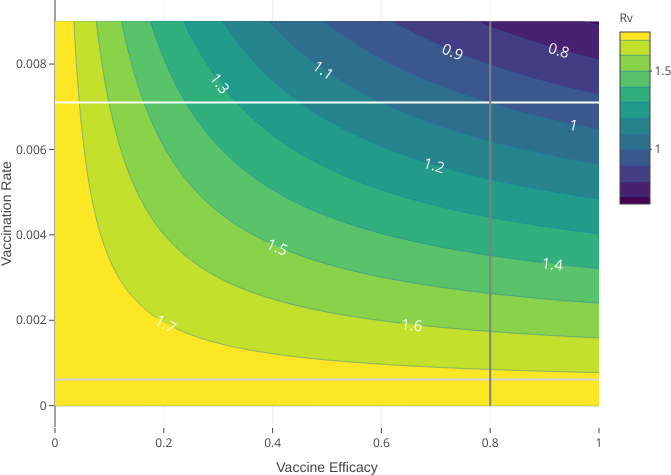
\includegraphics[scale=2.1, keepaspectratio]{Figures/R0_contour_1}
    \caption{R not contour plot as function of efficacy and vaccination rate.}
    \label{fig:r0contour1}
\end{figure*}


